\startchapter{Results}
\label{chapter:results}

In the last chapter, we detailed how we go about setting limits on the physics parameters in our scalar theory, from how we generate the raw events to extracting the upperbound on the coupling strength.
Here we will present our results, as the limits on the coupling as a function of mass for a new scalar particle, for the various experiments discussed previously.
This goes over the entire parameter space of $2m_e < m_\phi < (\sqrt{S_\textrm{Belle2}} - 2m_\tau)$, with different experiments taking different ranges of this total region.
For two of the cases, we've used \madgraph Monte Carlo techniques, and for the third scenario we've been able to analytically solve for the limits.
For all cases, our limits are a $3\sigma$ effect, as detailed in the previous section.
What we will plot below is the solution, $g_{\phi\mu}$, to the equation $S(m_\phi,g_{\phi\ell})/3\sqrt{B} = 1$, with $S \propto g_{\phi\mu}^2$, and the number of signal and background events being defined by the Monte Carlo or our hand calculations.
Specifically, since we know the scaling of the number of signal events (with each signal being defined in more detail below), we are solving the equation

\begin{equation}
\label{eqn:gphi_limit}
g_{\phi\mu}^\textrm{limit} = g_{\phi\mu}^\textrm{test} \left( \frac{S(m_\phi,g_{\phi\ell}^\textrm{test})}{3\sqrt{B}} \right)^{-1/2}
\end{equation}

\noindent for many masses over the parameter space, and where $g_{\phi\ell}^\textrm{test}$ is the appropriate input coupling used to generate the events.
This usually takes on a value of $0.1 - 1$.
Note that the form of the limit given in equation \ref{eqn:gphi_limit} will vary from experiment to experiment, as we take into account various things such as signal efficiency, however we always will end up solving this same equation.
Preemptively, we will show off our best limits here on the experiments to come in Fig.~\ref{fig:best_limits}.

\begin{figure}[h]
    \centering
    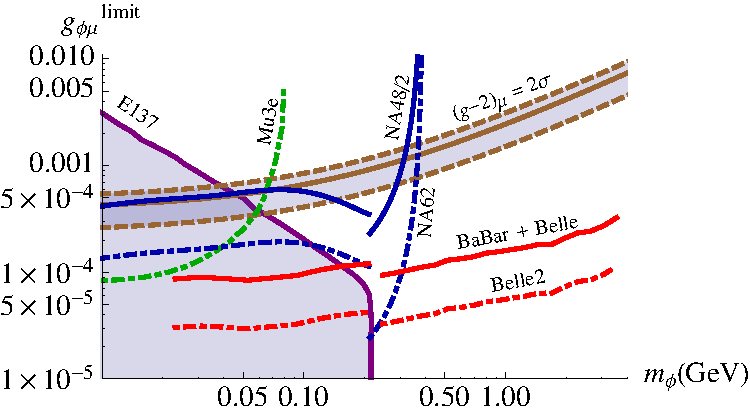
\includegraphics[width=0.8\textwidth]{Figures/limits/best_limits}
    \caption{Collection of the most promising limits as found by this work. Green shows the limits of phase II of \mueee, blue shows the upcoming NA62 experiment, and red shows the upgraded \belletwo experiment. See the rest of this chapter for details on the curves and how they are found.}
    \label{fig:best_limits}
\end{figure}

\input chapters/5/sec_muon
\input chapters/5/sec_kaon
\input chapters/5/sec_ee
